\section{Softwarearchitektur und Design}

\begin{concept}{Überblick Softwareentwicklung}
Die Entwicklung von Software erfolgt in verschiedenen Ebenen:
\begin{itemize}
    \item Business Analyse (Domänenmodell, Requirements)
    \item Architektur (Logische Struktur)
    \item Entwicklung (Konkrete Umsetzung)
\end{itemize}
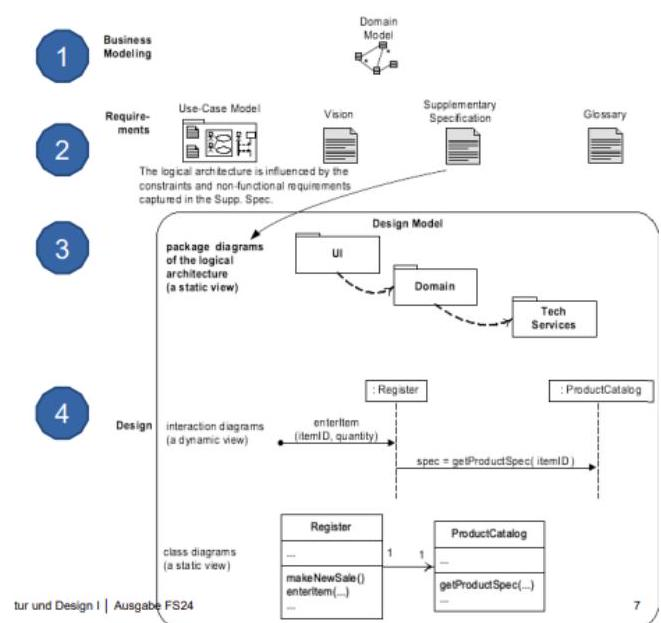
\includegraphics[width=0.9\linewidth]{images/2024_12_29_0d1d7b5551ea1b4b41bdg-07(2)}
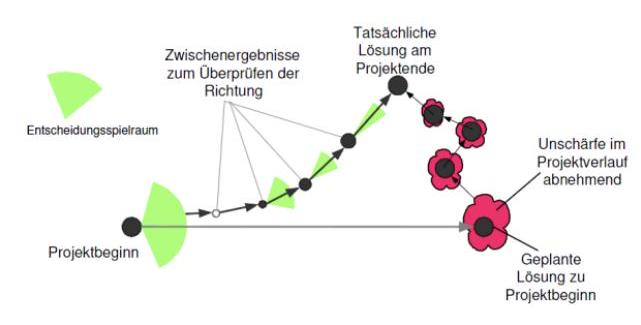
\includegraphics[width=0.9\linewidth]{images/2024_12_29_0d1d7b5551ea1b4b41bdg-08(1)}
\end{concept}

\begin{definition}{Softwarearchitektur}
Die Architektur definiert:
\begin{itemize}
    \item Grundlegende Strukturen und Komponenten
    \item Programmiersprachen und Plattformen
    \item Aufteilung in Teilsysteme und Bausteine
    \item Schnittstellen und deren Spezifikationen
    \item Basis-Technologien und Frameworks
    \item Besondere Maßnahmen für Anforderungserfüllung
\end{itemize}
\end{definition}

\begin{KR}{Architekturentscheidungen treffen}
\begin{enumerate}
    \item Anforderungen analysieren
    \begin{itemize}
        \item Funktionale Anforderungen identifizieren
        \item Nicht-funktionale Anforderungen priorisieren
        \item Randbedingungen berücksichtigen
    \end{itemize}
    
    \item Trade-offs evaluieren
    \begin{itemize}
        \item Performance vs. Flexibilität
        \item Skalierbarkeit vs. Komplexität
        \item Time-to-Market vs. Qualität
    \end{itemize}
    
    \item Architekturstil wählen
    \begin{itemize}
        \item Monolithisch
        \item Microservices
        \item Event-driven
        \item Layered
    \end{itemize}
    
    \item Entscheidungen dokumentieren
    \begin{itemize}
        \item Begründungen festhalten
        \item Alternativen aufzeigen
        \item Konsequenzen beschreiben
    \end{itemize}
\end{enumerate}
\end{KR}

[Previous content for Architekturanalyse remains...]

\begin{example}{Architekturentscheidungen}
Szenario: E-Commerce System
\begin{lstlisting}[language=Java]
// Monolithische Architektur
public class OrderService {
    private InventorySystem inventory;
    private PaymentSystem payment;
    private ShippingSystem shipping;
    
    public Order processOrder(Cart cart) {
        // Direkte Aufrufe
        if (inventory.checkStock(cart)) {
            Payment p = payment.process(cart.getTotal());
            shipping.schedule(cart.getItems());
            return new Order(cart, p);
        }
        throw new OutOfStockException();
    }
}

// Microservices Architektur
public class OrderService {
    private OrderRepository repository;
    private EventBus eventBus;
    
    public Order processOrder(Cart cart) {
        // Asynchrone Event-basierte Kommunikation
        Order order = repository.create(cart);
        eventBus.publish(new OrderCreatedEvent(order));
        return order;
    }
}
\end{lstlisting}
\end{example}

\begin{concept}{Modulkonzept}
Module werden nach zwei Hauptkriterien bewertet:

\textbf{Kohäsion (Zusammenhalt):}
\begin{itemize}
    \item Funktional: Alle Elemente tragen zu einer spezifischen Aufgabe bei
    \item Sequentiell: Ausgabe eines Elements ist Eingabe des nächsten
    \item Zeitlich: Elemente werden zur gleichen Zeit ausgeführt
    \item Logisch: Elemente gehören logisch zusammen
\end{itemize}

\textbf{Kopplung (Abhängigkeiten):}
\begin{itemize}
    \item Daten: Nur Datenaustausch
    \item Nachricht: Nur über definierte Schnittstellen
    \item Inhalt: Direkter Zugriff auf interne Daten
    \item Global: Gemeinsame globale Daten
\end{itemize}
\end{concept}

\begin{KR}{Modul-Design}
\begin{enumerate}
    \item Modul identifizieren
    \begin{itemize}
        \item Fachliche Zusammengehörigkeit
        \item Technische Abhängigkeiten
        \item Wiederverwendbarkeit
    \end{itemize}
    
    \item Schnittstellen definieren
    \begin{itemize}
        \item Exportierte Services
        \item Benötigte Services
        \item Datenformate
    \end{itemize}
    
    \item Interne Struktur entwerfen
    \begin{itemize}
        \item Klassen und Komponenten
        \item Datenstrukturen
        \item Algorithmen
    \end{itemize}
\end{enumerate}
\end{KR}

[Previous content for N+1 View Model and UML sections remains...]

\begin{example}{UML-Modellierung in der Praxis}
Modellierung eines Bestellsystems:

\textbf{1. Statisches Modell (Klassendiagramm):}
\begin{lstlisting}[language=Java]
public class Order {
    private List<OrderItem> items;
    private Customer customer;
    private OrderStatus status;
    
    public BigDecimal calculateTotal() { ... }
    public void addItem(Product p, int qty) { ... }
}

public class OrderItem {
    private Product product;
    private int quantity;
    private BigDecimal price;
}
\end{lstlisting}

\textbf{2. Dynamisches Modell (Sequenzdiagramm Code):}
\begin{lstlisting}[language=Java]
// Prozess der im Sequenzdiagramm dargestellt wird
public class OrderProcess {
    public void processOrder(Order order) {
        // 1. Validierung
        validateOrder(order);
        
        // 2. Reservierung
        inventory.reserve(order);
        
        // 3. Zahlung
        payment.process(order);
        
        // 4. Bestätigung
        notifyCustomer(order);
    }
}
\end{lstlisting}
\end{example}

[Previous content for RDD and GRASP remains...]

\begin{KR}{Anwendung von GRASP-Prinzipien}
\begin{enumerate}
    \item Information Expert
    \begin{itemize}
        \item Identifiziere benötigte Informationen
        \item Finde Klasse mit dieser Information
        \item Weise Verantwortlichkeit zu
    \end{itemize}
    
    \item Creator
    \begin{itemize}
        \item Prüfe Beziehungen zwischen Klassen
        \item Wähle stärkste Beziehung
        \item Weise Erstellungsverantwortung zu
    \end{itemize}
    
    \item Low Coupling/High Cohesion
    \begin{itemize}
        \item Analysiere Abhängigkeiten
        \item Gruppiere zusammengehörige Funktionalität
        \item Minimiere externe Abhängigkeiten
    \end{itemize}
\end{enumerate}
\end{KR}